%******************************************************************************%
%                                                                              %
%                  sample.en.tex for LaTeX                                     %
%                  Made by : Michael Lu (mlu@student.42.fr)                    %
%                                                                              %
%******************************************************************************%

\documentclass{42-en}


%******************************************************************************%
%                                                                              %
%                                    Header                                    %
%                                                                              %
%******************************************************************************%
\begin{document}



                           \title{ft\_arena}
                          \subtitle{Introductory Object Oriented Programming}
                       \member{Michael Lu}{mlu@student.42.fr}
\summary {
  This project is about creating fighters who will battle it out in the arena
}

\maketitle

\tableofcontents


%******************************************************************************%
%                                                                              %
%                                  Foreword                                    %
%                                                                              %
%******************************************************************************%
\chapter{Foreword}

	Have you ever wondered how to write and structure your own game?\\

	A game infamous for having a very talent team of programmers but
	failed to execute is IMC Games, the producers who created the new
	MMORPG Tree of saviors. This team contained developers from a team
	called Gravity which was famous for Ragnarok Online, a old school
	2.5d MMORPG that had an emphasis on social play. So what went wrong
	with tree of saviors?\\

	IMC Games had previewed alot of crazy cool stuff like having four main
	class that can branch into multitude of classes. Boasting eight new classes
	(two for each four main class) at each rank (currently at nine ranks), 
	you had 76 different classes! Imagine being able to build any kind of class
	you wanted with those combinations! However, it was only but a dream.\\

	Sure they succeeded in implementing this cool idea, but they had alot of
	optimization issue and balancing issues. There were constant server problems,
	latency and imbalanced classes that slowly dwindled the player community.
	By the time the developers had fixed up majority of the optimization issue,
	balancing issue and server issues the damage has been done. Most of the hype
	was gone and many gamers had moved onto other MMORPGs. Was it how they written
	the game that killed it? Maybe it was their structure? Who knows.\\

	As someone who still players Tree of Savior I hope this tidbit gives you some
	interested insight.

	\begin{center}
		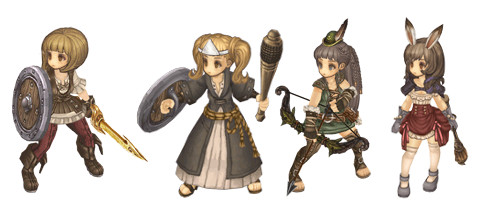
\includegraphics[width=0.8\textwidth]{images/classes.jpg}
	\end{center}

%******************************************************************************%
%                                                                              %
%                                 Introduction                                 %
%                                                                              %
%******************************************************************************%
\chapter{Introduction}

	The goal of this project is to create a fun arena simulator where you
	your own characters who will fight for the death! Let's be real,
	it's exciting to make a game and learn the skills to do so, but it's
	important to start with the basic. What are classes? What is inheritance?
	Did you know that ruby and python has almost everything as objects/classes?
	I bet you didn't know that, and for that reason makes the language unique
	from others.\\

	\warn{
		If you are using python or another language approved by hack high school
		 make sure to research into python equivalent
		concepts on your own. This project can be completed in any
		 approve project language,
		however the tutorial and video guides will be in Ruby.
	}

	So how do you even start making an arena simulator? Simple. First, you
	need to contain information for your fighters. Second, you need to make
	every fighter unique. It'd be boring if they all did the same thing. 
	Lastly, you need to make them fight. And guess what? All of this can be done
	using object oriented programming. After you learn classes you'll never
	go back. The skills you learn from this will only help you should you choose
	to do any other projects, as using classes can easily help you scale
	and complete more difficult projects. So let's start with the basics first.\\



%******************************************************************************%
%                                                                              %
%                                  Goals                                       %
%                                                                              %
%******************************************************************************%
\chapter{Goals}

	The goal of ft\_arena is to introduce you into basic object oriented programming.
	By the end of this project you should know how to:\\
	
	\begin{itemize}
		\item Design classes (parent, children, etc)
		\item Utilize inheritances
		\item Utilize multiple classes
		\item Create class interactions
		\item Be awesome\\
	\end{itemize}
	 
	You will be exploring a fundamental topic of object oriented programming
	so take advantage of all the resources including the video, your neighbor
	and google. There are many tutorials on classes and inheritance.


%******************************************************************************%
%                                                                              %
%                             General instructions                             %
%                                                                              %
%******************************************************************************%
\chapter{General instructions}

	    \begin{itemize}
		\item This project will only be corrected by actual human beings.
		You are therefore free to organize and name your files as you wish,
		although you must respect some requirements listed below
		\item Your must have a parent class and a children class (they do not
		need to be named parent/children, but it should be easy to see
		which is the children and which is the parent)
		\item A container class is optional but highly recommended
		
		\hint{
			It will help you alot to practice writing your parent and
			children class first. After you can focus on writing
			your container or main and storing your classes.
			I recommend a container with an array to store your classes.
			You can see this demo in the tutorial video. There are
			other ways to store your classes so feel free to choose
			what you feel most comfortable with.
		}	
				
		
		\item Your project must be written in a language approved by
		the hack high school program
		\item You must create at least three unique children class
		\item You must have a menu/selection screen for people to choose
		the name and class/job/specialization of your fighter
		\item You must allow the ability for people to pick which fighter
		they want to have fight against eachother in the arena
		\item You must use at least two variables for the parent class:
		health and attack. You can shorten these names or rename them, but
		you must have some sort of health and attack variable
		\item Ask your peers, mentor, slack or anywhere else if you need
		any help, and make sure to have fun\\
	\end{itemize}



%******************************************************************************%
%                                                                              %
%                             Mandatory part                                   %
%                                                                              %
%******************************************************************************%
\chapter{Mandatory part}

	\begin{itemize}
		\item The goal of this project is to create a simple program
		that will take two fighters and make them fight eachother
		\item All fights will be one on one, so do not worry about having
		more than two fighters fighting eachother at the same time
		\item At the beginning of the program the users should have a menu
		that allows them to create a fighter, start a fight in the arena,
		and to see all the fights available (any extra stuff is fine)

	\begin{center}
		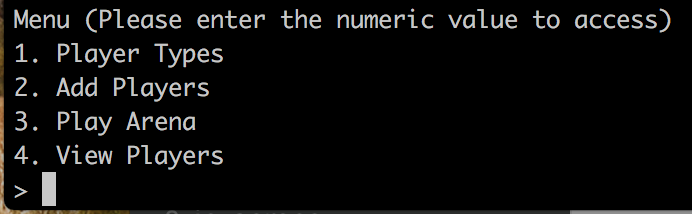
\includegraphics[width=0.6\textwidth]{images/menu.png}
	\end{center}

		\item Only health and attack is required variable for the fighters,
		feel free to add any other variables if needed
		\item When the user chooses to have fighters fight in the arena
		they must be able to select two unique fighters. The fighter cannot
		be the same fighter.
		\item You can choose to reset the fighter after the fight, or leave
		them weaken/incapacitated from their previous fight. It is not required
		to have all the fighters fully heal for the next fight.
		\item You must display all the fights out to the terminal

	\begin{center}
		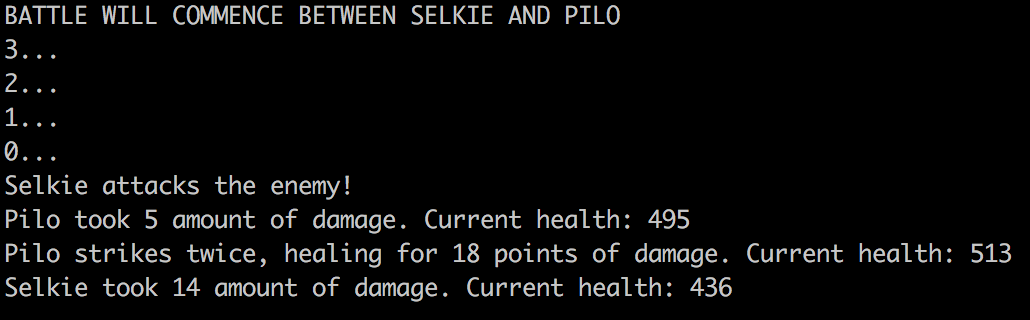
\includegraphics[width=0.6\textwidth]{images/fight.png}
	\end{center}

		\item It should be clear in the terminal who is attacking and who
		is taking damage
		\item When a fighter's health reaches zero the fight is over and the victor
		must be declared in the terminal.
		\item When the fight is over you must have the user redirected back
		to the main menu where they can create more fighters or do more fights

		\hint{
			How you structure your while loops, and if/else, case switch,
			hash table, etc. Can make or break your menu. Consider
			designing something simple that is easy to repeatedly call
			the menu and easy to add stuff onto the menu.
		}

		\item You should try to make the user experience as enjoyable as
		possible. For this reason the user should be able to see all created
		fighter so they can pick them for the arena fights.
		\item Because you are simulating a simple arena fight make sure
		you delay your terminal output. Having the entire battle post
		immediately to the terminal instantly is not okay.
		\item You must handle any kind of user error to the best of your
		ability. The most vital one is to make sure there is no error in
		creating a character, and there is at least two viable fighters
		to put into the arena together.
		
	\end{itemize}

%******************************************************************************%
%                                                                              %
%                                 Bonus part                                   %
%                                                                              %
%******************************************************************************%
\chapter{Bonus part}
	
	Remember this is a simple self automated simulator, kind of like a game.
	For this reason there are many things you can do for bonus. Feel
	free to add whatever you'd like to spice up your program as long as
	you meet all the requirements above. Some things you could try out
	for bonuses are listed below:

	\begin{itemize}
		\item Sound effects
		\item Additional classes
		\item Cool text/color effects in terminal
		\item Any visualizer
		\item An amazing game container that holds all their classes
		\item Unique skills, attributes or stats
		\item Additional mechanics, or randomness to the fight 
		\item Any other cool features you can come up with to enhance
		your simulator!	
	\end{itemize}



%******************************************************************************%
%                                                                              %
%                           Turn-in and peer-evaluation                        %
%                                                                              %
%******************************************************************************%
\chapter{Turn-in and peer-evaluation}

    Turn your work in using your \texttt{GiT} repository, as
    usual. Only work present on your repository will be graded in defense.\\

	Good luck and remember to have fun!



%******************************************************************************%
\end{document}
